
% COVER PAGE
\begin{titlepage}
\newgeometry{top=3cm, bottom=3cm,
			left=2.25 cm, right=2.25cm}	% Temporarily change margins

% Cover page background
\AddToShipoutPicture*{\backgroundpic{-4}{56.7}{figure/auxiliary/frontpage_swe.pdf}}
\addtolength{\voffset}{2cm}

% Cover picture
\begin{figure}[H]
\centering
\vspace{0cm}	% Adjust vertical spacing here
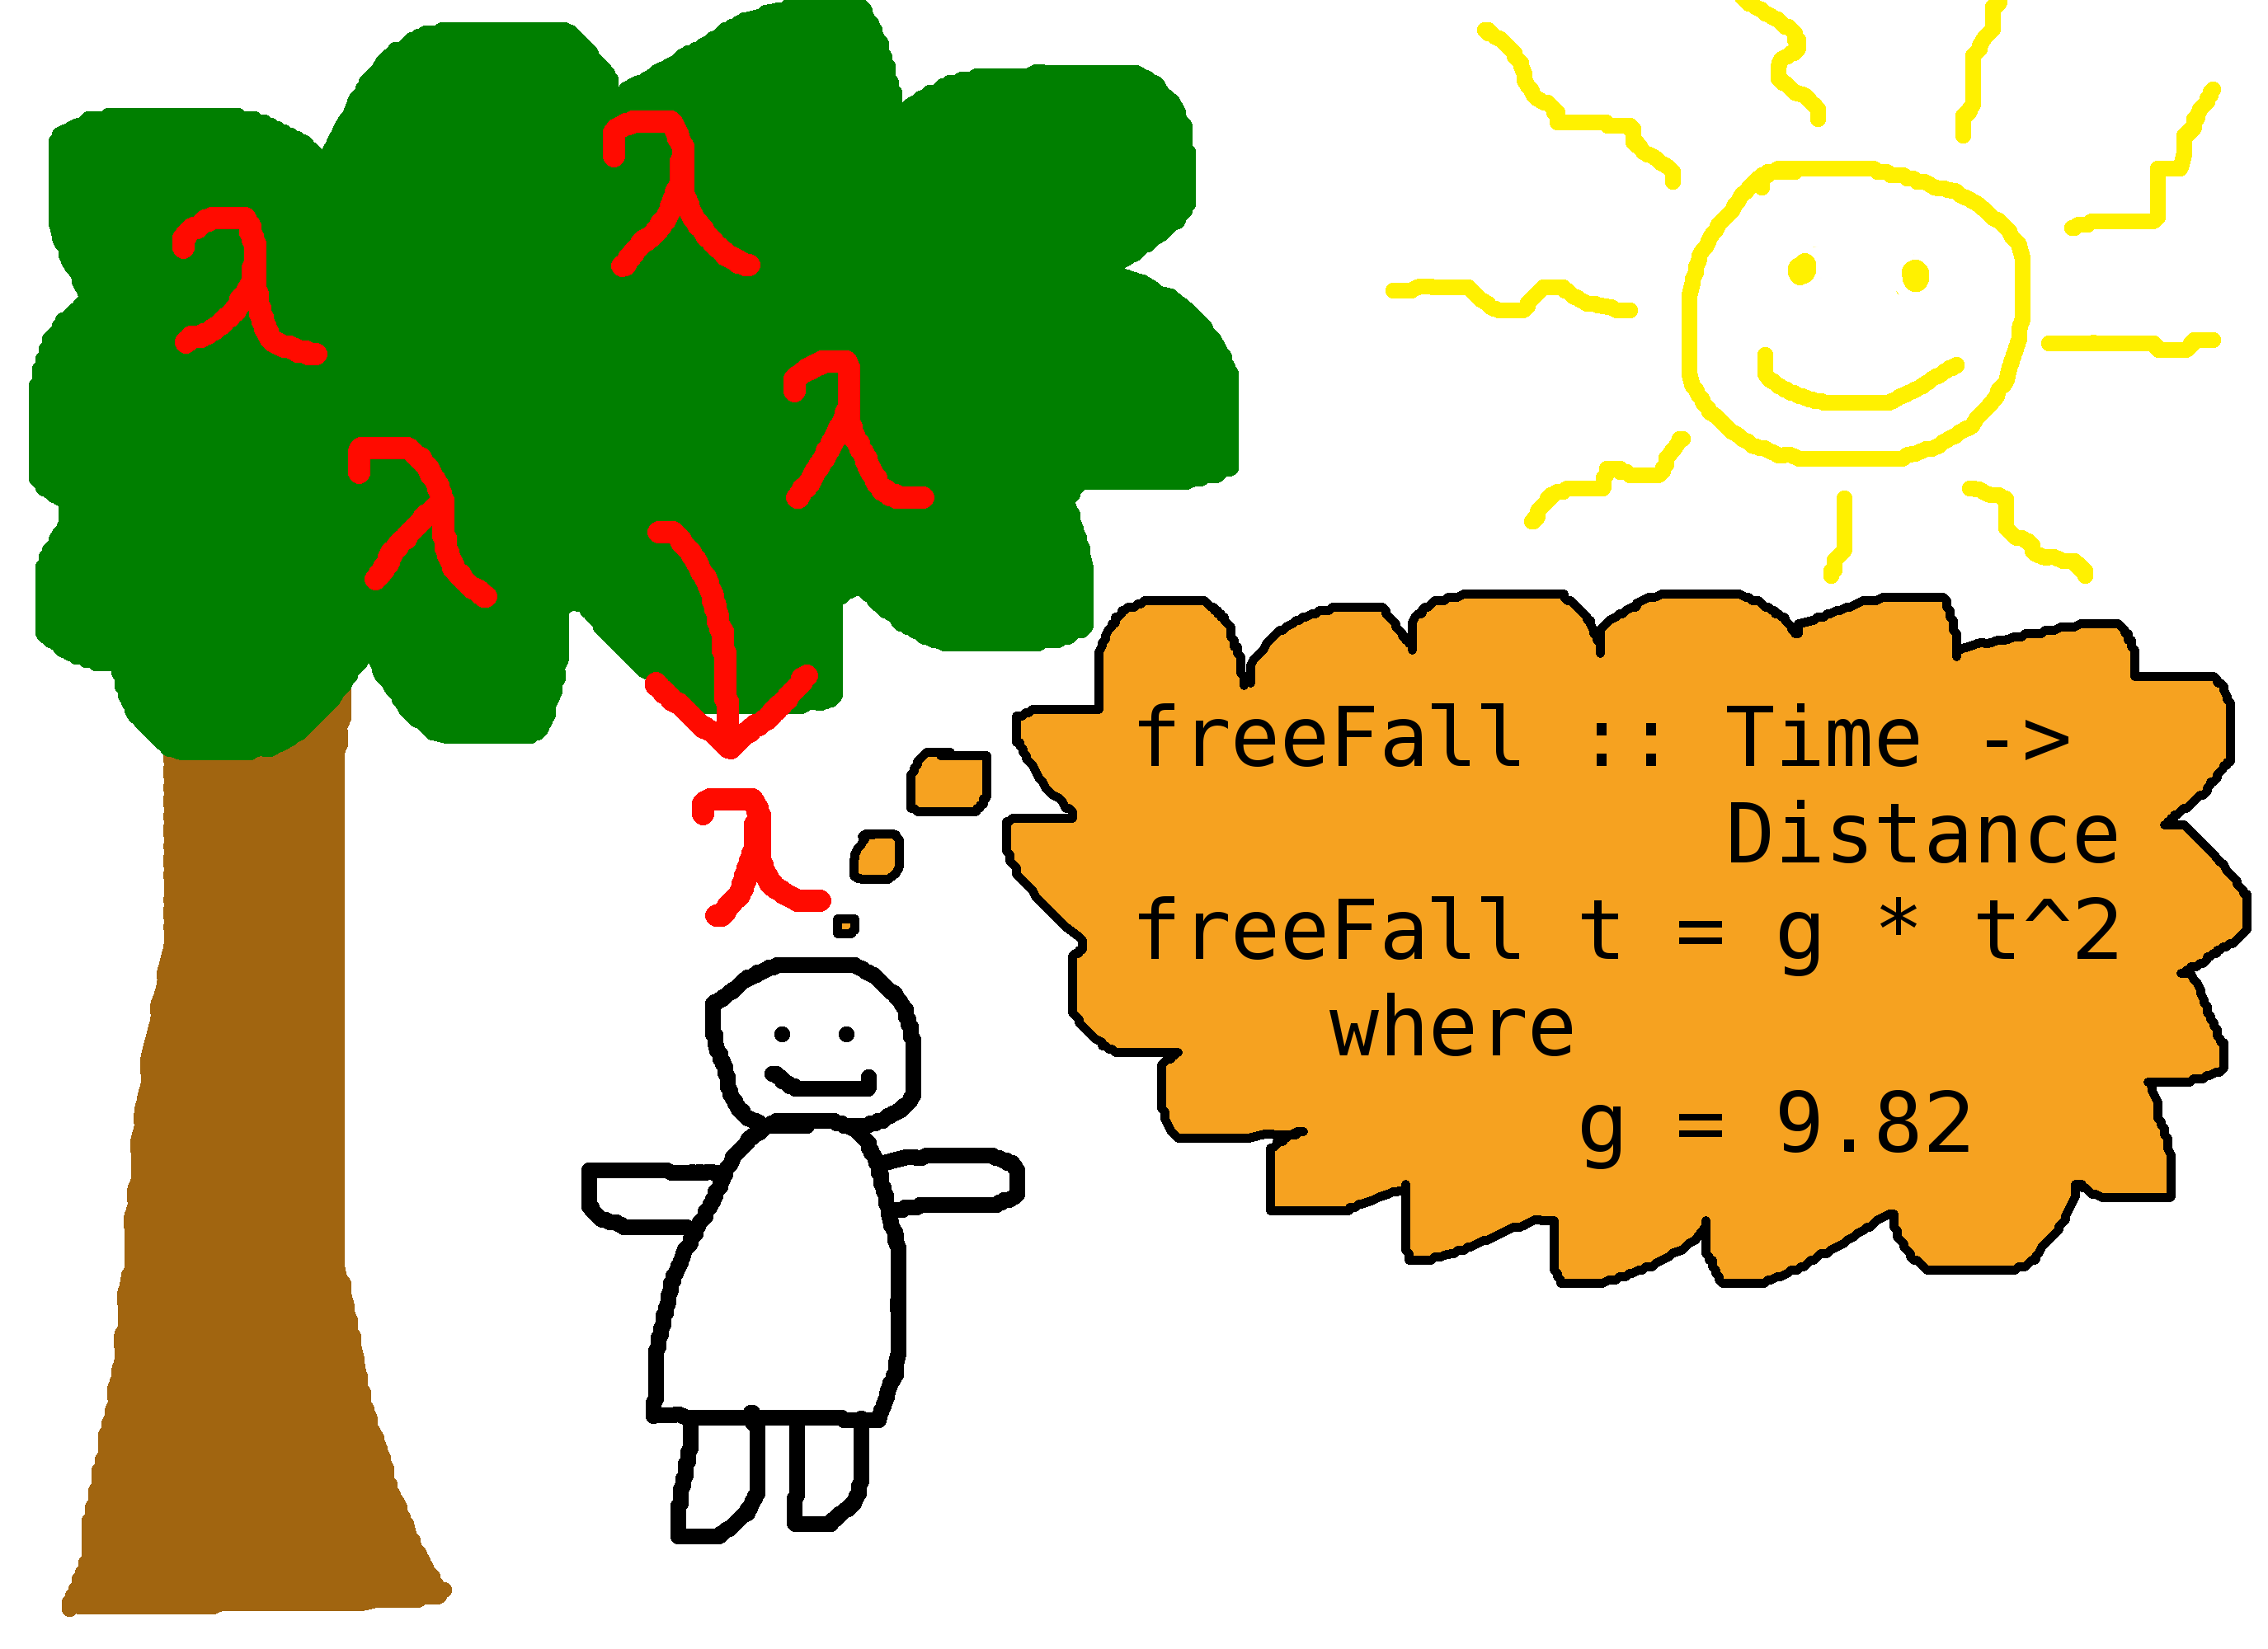
\includegraphics[width=0.99\linewidth]{figure/Framsida.png}
\end{figure}

% Cover text
%\mbox{}
%\vspace{2cm}
\renewcommand{\familydefault}{\sfdefault} \normalfont % Set cover page font
\vfill
\textbf{{\Huge  Ett alternativt läromaterial för data-\\studenter som lär sig fysik}} 	\\[0.5cm]
{\Large Läromaterialet Learn You a Physics for Great Good!}\\[0.5cm]
Kandidatarbete inom Data- och informationsteknik
\setlength{\parskip}{1cm}

{\Large Johan Johansson \\[0.3cm]
Oskar Lundström \\[0.3cm]
Erik Sjöström \\[0.2cm]
Björn Werner \\[0.2cm]}

Institutionen för Data- och informationsteknik \\
\textsc{Chalmers tekniska högskola} \\
Göteborg, Sverige 2018

\renewcommand{\familydefault}{\rmdefault} \normalfont % Reset standard font
\end{titlepage}


% BACK OF COVER PAGE (BLANK PAGE)
\newpage
\restoregeometry
\thispagestyle{empty}
\mbox{}


% TITLE PAGE
\newpage
\thispagestyle{empty}
\begin{center}
	\textsc{\large Kandidatarbete DATX02-18-08}\\[4cm]		% Report number given by department
	\textbf{\Large Ett alternativt läromaterial för datastudenter som lär sig fysik} \\[1cm]
	{\large Läromaterialet Learn You a Physics for Great Good!}\\[1cm]
	{\large Johan Johansson}\\
  {\large Oskar Lundström}\\
 	{\large Erik Sjöström}\\
  {\large Björn Werner}\\

	\vfill
	% Logotype on titlepage
	\begin{figure}[H]
	\centering
	% Remove the following line to remove the titlepage logotype
	
\includegraphics[width=0.2\pdfpagewidth]{figure/auxiliary/logo_swe.pdf} \\
	\end{figure}	\vspace{5mm}

	Institutionen för Data- och informationsteknik \\
	\emph{Avdelningen för funktionell programmering}\\
	\textsc{Chalmers tekniska högskola} \\
	Göteborg, Sverige 2018 \\
\end{center}


% IMPRINT PAGE (BACK OF TITLE PAGE)
\newpage
\thispagestyle{plain}
\vspace*{0cm}
Ett alternativt läromaterial för datastudenter som lär sig fysik\\
Läromaterialet Learn You a Physics for Great Good!\\
Johan Johansson \\
Oskar Lundström \\
Erik Sjöström \\
Björn Werner
\setlength{\parskip}{1cm}

\copyright ~ Johan Johansson, 2018. \setlength{\parskip}{1cm} \\
\copyright ~ Oskar Lundström, 2018. \setlength{\parskip}{1cm} \\
\copyright ~ Erik Sjöström, 2018. \setlength{\parskip}{1cm} \\
\copyright ~ Björn Werner, 2018. \setlength{\parskip}{1cm}

Handledare: Patrik Jansson, CSE, Chalmers\\
Examinator: Nils Anders Danielsson, CSE, Chalmers \setlength{\parskip}{1cm}

Kandidatarbete DATX02-18-08 \\
Institutionen för Data- och informationsteknik \\
Avdelningen för funktionell programmering\\
Chalmers tekniska högskola\\
SE-412 96 Göteborg\\
Telefon +46 31 772 1000
\setlength{\parskip}{0.5cm}%TODO: why set it here?

\vfill
% Caption for cover page figure if used, possibly with reference to further information in the report
Omslag: Newton står och tänker på fritt fall i termer av Haskellkod och precis då får han ett lambda-äpple i huvudet. Bilden är ritad i samma stil som bilderna i läromaterialet.

Typsatt i \LaTeX \\
Göteborg, Sverige 2018
